Determining the structure of a typical $H$-free graph is a problem at the heart of combinatorics.
Because it lies at the interface of several subjects including asymptotic enumeration, extremal graph theory, and nonlinear large deviations, the problem has bridged different areas and given new perspectives on classical results.
An example is the \citeyear{erdos1976enumeration} theorem of \citeauthor{erdos1976enumeration} \cite{erdos1976enumeration} stating that almost all triangle-free graphs are bipartite. This theorem introduced the idea that typical $H$-free graphs closely resemble a subgraph of an extremal $H$-free graph. In the case of triangle-free graphs, Mantel's theorem \cite{mantel1907vraagstuk} states that the extremal structure is complete balanced bipartite.
Powerful results have since shown that the asymptotic enumeration and typical structure of graph properties often reduce to a related optimization problem. This paper is about the solution to a graphon variational problem and a finer counting argument that yield a precise structural description of typical graphs of given density not containing an induced star.

A graph is \emph{induced-$H$-free} if none of its induced subgraphs is isomorphic to $H$. \citeauthor{promel1991excluding} pioneered the study of typical induced-$H$-free graphs in papers on induced-$C_4$-free graphs \cite{promel1991excluding} and induced-$C_5$-free graphs \cite{promel1992almost}. These papers are notable for determining the first-order asymptotics of the number of graphs in question. \citeauthor{promel1992excluding} \cite{promel1992excluding} also determined the first-order asymptotics of the logarithm of the number of induced-$H$-free graphs for \emph{all} $H$ in terms of the coloring number of $H$, a quantity we define below. \citeauthor{alekseev1993entropy} \cite{alekseev1993entropy} and \citeauthor{bollobas1997hereditary} \cite{bollobas1997hereditary} generalized this to hereditary properties, and \citeauthor{alon2011structure} \cite{alon2011structure} strengthened it to a rough structure result for hereditary properties. \citeauthor{balogh2011excluding} \cite{balogh2011excluding} proved a precise typical structure result for all $H$ that satisfy a certain notion of criticality, and this has been extended by \citeauthor{norin2025typicalI} \cite{norin2025typicalI,norin2025typicalII}. Detailed typical structure results have also been proven for induced-$C_{2\ell}$-free graphs \cite{kim2018forbidding} and induced-$(K_{a+b}\setminus K_b)$-free graphs \cite{keevash2017structure}.

The typical structure of $H$-free graphs with a given number of edges $m=m(n)$ was also first studied by \citeauthor{promel1996asymptotic}. Refining \erdos{}--Kleitman--Rothschild, they proved that if $m=\Omega(n^{7/4}\log n)$ then almost all triangle-free graphs on $n$ vertices and $m$ edges are bipartite \cite{promel1996asymptotic}. Today, the typical structure of triangle-free graphs \cite{osthus2003densities,steger2005evolution,stark2018probability,jenssen2025evolution} and more generally $K_{r+1}$-free graphs \cite{luczak2000triangle,balogh2009typical,balogh2015independent,balogh2016typical} with $m$ edges are well understood. By contrast, induced-$H$-free graphs with $m$ edges have received much less attention. \citeauthor{bottcher2012perfect} \cite{bottcher2012perfect} proved that induced-$C_5$-free graphs and perfect graphs of fixed constant density have the same exponential growth rate. \citeauthor{morris2024asymmetric} \cite{morris2024asymmetric} proved that if $n^{4/3}(\log n)^4\leq m \leq o(n^2)$ then almost all induced-$C_4$-free graphs with $m$ edges are within $o(m)$ edit distance of a split graph, while if $m=o(n^{4/3}(\log n)^{1/3})$ then this is not the case. Recently, Perkins and the author \cite{perkins2025typical} proved that claw-free graphs of fixed constant edge density exhibit a phase transition, characterized the optimizers of the associated graphon variational problem, and proved detailed typical structure results.

From another perspective, conditioning the \erdosrenyi{} random graph $G(n,p)$ to be $H$-free places the problem in lower-tail large deviations for subgraph counts. Writing $X_H$ for the number of copies of $H$ in $G(n,p)$, the lower-tail event is $X_H\leq(1-\eta)\E X_H$ for a parameter $0<\eta\leq1$.
A seminal result of \citeauthor{chatterjee2011large} \cite{chatterjee2011large} implies as a special case that for constant $p$, the lower-tail \emph{rate function} (i.e.\ the constant in the leading term of the exponent of the lower-tail probability) is given by a variational problem over graphons.
\citeauthor{zhao2017lower} \cite{zhao2017lower} proved that the lower-tail variational problem exhibits a phase transition in the sense of a non-analyticity of the rate function in $p$ and $\eta$: for small $\eta$, the optimizer is constant, while for $\eta$ close to 1, this is not the case. A full characterization of the optimizers for all $p$ and $\eta$ remains a difficult open problem, even for triangles. \citeauthor{kozma2023lower} \cite{kozma2023lower} proved that the lower-tail rate function is still given by a variational problem down to $p=\Omega(n^{-1/m_2(H)})$, where $m_2(H)$ is the 2-density
of $H$, which is the full range of densities where the reduction could hold. A similar reduction for the rate function of the lower tail for \emph{induced} copies is only known in the dense setting due to \citeauthor{chatterjee2011large}.

In this paper, we completely solve the variational problem over graphons with zero induced $K_{1,k}$ density and fixed constant edge density. The solution yields the entropy density of induced-$K_{1,k}$-free graphs of given edge density, the large deviation rate function for induced-$K_{1,k}$-freeness in $G(n,p)$ for constant $p$, and a rough structural description of both random graph models. Most notably, the variational problem exhibits a phase transition that is second-order in the fixed-density model and first-order in the conditioned \erdosrenyi{} random graph. Both models have infinitely many optimal graphons for some parameter values, but there is always a unique graphon that represents the typical structure in cut metric. A more detailed analysis of the counts and probabilities yields a finer structural characterization of a typical sample from each model. Finally, we show that the induced-$H$-free fixed-density variational problem does not necessarily exhibit a phase transition in general: we prove that almost all induced-$C_4$-free graphs of fixed constant edge density are split graphs, resolving the dense case of a conjecture of \citeauthor{morris2024asymmetric} \cite[Conjecture~6.1]{morris2024asymmetric} and refining a theorem of \citeauthor{promel1991excluding} \cite{promel1991excluding}.

\subsection{Main results}
For a graph $H$, let $\cF^\ast_{n,m}(H)$ be the set of induced-$H$-free graphs on $n$ vertices and $m$ edges, and let $N^\ast_{n,m}(H):=\abs{\cF^\ast_{n,m}(H)}$. The \emph{entropy density} of a property $\cP(n)$ of graphs is defined as $\lim_{n\to\infty}\binom{n}{2}^{-1}\log|\cP(n)|$, and its \emph{large deviation rate function} is defined as $-\lim_{n\to\infty}\binom{n}{2}^{-1}\log\bbP\{G(n,p)\in\cP(n)\}$, provided the limits exist. For an integer $r\geq2$, a graph is \emph{co-$r$-partite} if it is the complement of an $r$-partite graph.

Our first main result establishes the entropy density of $\cF^\ast_{n,m}(K_{1,k})$ for $m=\Theta(n^2)$. For every integer $k\geq3$, let $p_k\in(0,1)$ be the unique solution to the equation $p_k=(1-p_k)^{k-1}$. Define the constant
\begin{equation}\label{eqn:gammak-dfn}
\gamma_k:=\frac{1+(k-2)p_k}{k-1}
\end{equation}
and define the function $\sE_k:[0,1]\to\R$ by
\begin{equation}\label{eqn:entropy-dfn}
\sE_k(x):=\begin{cases}\frac{(k-2)x}{1+(k-2)p_k}\,H(p_k)&0\leq x\leq\gamma_k\\[5pt]\big(1-\frac{1}{k-1}\big)\,H\!\left(\frac{(k-1)x-1}{k-2}\right)&\gamma_k\leq x\leq1\end{cases}\,,
\end{equation}
where $H(x)=-x\log x-(1-x)\log(1-x)$ is the binary entropy. The notation $f(n)\sim g(n)$ means $\lim_{n\to\infty}f(n)/g(n)=1$.

\begin{theorem}\label{thm:main-entropy}
Fix constants $k\geq3$ and $\gamma\in(0,1)$. If $m\sim\gamma\binom{n}{2}$ then
\begin{equation*}
\lim_{n\to\infty}\frac{1}{\binom{n}{2}}\log N^\ast_{n,m}(K_{1,k})=\sE_k(\gamma) \,.
\end{equation*}
\end{theorem}

The graph of $\sE_k$ is shown on the left axis of \Cref{fig:rate-funcs} for several values of $k$. Since $\sE_k$ has a continuous first derivative and a discontinuous second derivative at $\gamma_k$, the uniformly random graph $G\in\cF^\ast_{n,m}(K_{1,k})$ is said to exhibit a \emph{second-order phase transition} at edge density $\gamma_k$. See \cite{jaeger1998ehrenfest} for background on the Ehrenfest classification of phase transitions. To understand the entropy density $\sE_k(\gamma)$, note that the concave piece on the interval $[\gamma_k,1]$ is the entropy density of co-$(k-1)$-partite graphs of edge density $\gamma+o(1)$, while the linear piece on the interval $[0,\gamma_k]$ is the entropy density of graphs of edge density $\gamma+o(1)$ that are the disjoint union of a co-$(k-1)$-partite graph and an empty remainder.

In the next theorem, we present the rate function for induced-$K_{1,k}$-freeness. For all $k\geq3$ define the function $\sR_k:[0,1]\to\R$ by
$$\sR_k(x):=\begin{cases}\log(\frac{1}{1-x})&0\leq x\leq p_k\\[4pt]\frac{1}{k-1}\log(\frac{1}{x})&p_k\leq x\leq1\end{cases}\,.$$
Let us write $H\leq G$ to declare that $H$ is an induced subgraph of $G$.

\begin{theorem}\label{thm:main-rate}
Fix constants $k\geq3$ and $p\in(0,1)$. Then
\begin{equation*}
\lim_{n\to\infty}\frac{1}{\binom{n}{2}}\log\bbP\{G(n,p)\not\geq K_{1,k}\}=-\,\sR_k(p) \,.
\end{equation*}
\end{theorem}

To understand the rate function $\sR_k(p)$, note that the supercritical piece on $[p_k,1]$ is the rate function for the event that $G(n,p)$ is co-$(k-1)$-partite, while the subcritical piece on $[0,p_k]$ is the rate function for the event that $G(n,p)$ is empty. In fact, \Cref{thm:main-rate} can be read off from results of \citeauthor{thomason2011graphs} \cite{thomason2011graphs} (specifically, by combining Theorem 4.4 and Section 7.5), who studied extremal problems that complement those of this paper. Connections to this prior literature are discussed further below.

\begin{figure}
	\begin{center}
	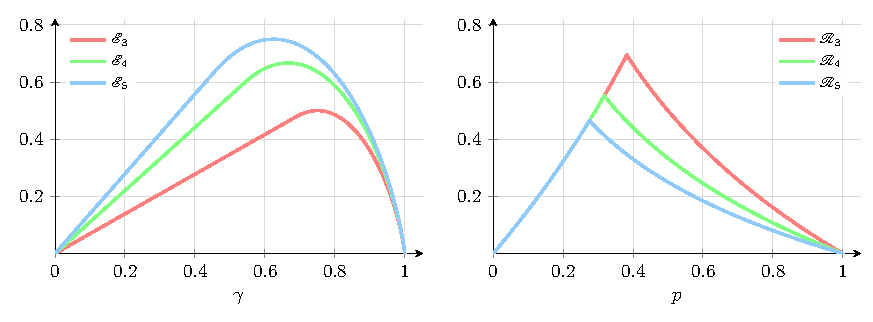
\includegraphics{Graphics/rate-functions.pdf}
	\end{center}
	\caption{The entropy density $\sE_k$ (left) and rate function $\sR_k$ (right) for $k=3,4,5$. The curves $\sR_3$, $\sR_4$, and $\sR_5$ coincide on the interval $[0,p_5]$.}
	\label{fig:rate-funcs}
\end{figure}

The most important feature of both \Cref{thm:main-entropy,thm:main-rate} is that the entropy density and rate function are given by piecewise formulas, reflecting that there are competing structural mechanisms that determine the exponential rates. These competing structures were heuristically described above by noting that the entropy densities or rate functions match the formulas given in $\sE_k$ and $\sR_k$. Our next set of results show that, in fact, these heuristics precisely characterize the typical structure of the corresponding random graph models.

Here and throughout, \emph{almost all} and \emph{almost every} mean all but a $o(1)$ fraction.

\begin{theorem}\label{thm:main-almostall}
Fix $k\geq3$. The following hold:
\begin{enumerate}[
  label=\textit{(\roman*)},
  ref=(\textit{\roman*}),
  topsep=5pt
]
	\item\label{item:thm:main-almostall-super} Fix $\gamma\in(\gamma_k,1)$. If $m\sim\gamma\binom{n}{2}$ then almost every $G\in\cF^\ast_{n,m}(K_{1,k})$ is co-$(k-1)$-partite.
	\item\label{item:thm:main-critical} Let $a_\ast:=\frac{(k-2)p_k(1-p_k)\ln2}{(k-1)\gamma_k}$ and fix $a\in\R$. Let
	$$\gamma:=\gamma_k+a\frac{\log n}{n}$$
	and set $m:=\floor{\gamma\binom n2}$. If $a\leq a_\ast$ then almost every $G\in\cF^\ast_{n,m}(K_{1,k})$ is the disjoint union of two graphs $G=G_1\sqcup G_2$ such that $G_1$ is co-$(k-1)$-partite and
	$$v(G_2)=\left(\frac{a_\ast-a}{2\gamma_k}+o(1)\right)\log n\,.$$
	If $a>a_\ast$ then almost every $G\in\cF^\ast_{n,m}(K_{1,k})$ is co-$(k-1)$-partite.
	\item\label{item:thm:main-almostall-sub} Fix $\gamma\in(0,\gamma_k)$. If $m\sim\gamma\binom{n}{2}$ then almost every $G\in\cF^\ast_{n,m}(K_{1,k})$ is the disjoint union of two graphs $G=G_1\sqcup G_2$ such that $G_1$ is a co-$(k-1)$-partite graph on
	$$(1+o(1))\left(\frac{\gamma(k-1)}{1+(k-2)p_k}\right)^{1/2}n\,,$$
	vertices and $G_2$ is a graph with $\Omega(n)\leq e(G_2)\leq o(n^2)$ edges.
\end{enumerate}
\end{theorem}

For $\gamma\in(\gamma_k,1)$, \Cref{thm:main-almostall} \ref{item:thm:main-almostall-super} significantly strengthens \Cref{thm:main-entropy} since it gives the first-order asymptotics of $N^\ast_{n,m}(K_{1,k})$: letting $r=k-1$ and assuming $r\mid n$, the number $C^r_{n,m}$ of co-$r$-partite graphs on $n$ vertices and $m\sim\gamma\binom{n}{2}$ edges is
$$C^r_{n,m}=(1+o(1))\vast(\sum_{\substack{z_1,\dots,z_r\in\mathbb Z\\ z_1+\cdots+z_r=0}}
\left(\frac{r\gamma-1}{r-1}\right)^{\frac12(z_1^2+\cdots+z_r^2)}\vast)\,\frac{1}{r!}\,
\binom{n}{\frac{n}{r},\dots,\frac{n}{r}}
\binom{\binom{r}{2}\frac{n^2}{r^2}}{\,m-r\binom{n/r}{2}}\,.$$
Meanwhile, in the subcritical regime in \Cref{thm:main-almostall} \ref{item:thm:main-almostall-sub}, there is a nonempty \emph{sparse} remainder on $\Theta(n)$ vertices outside the co-$(k-1)$-partite core.

The next main result describes the typical structure of the conditioned \erdosrenyi{} random graph $G(n,p)$ for constant $p$, where we again observe a structural dichotomy.

\begin{theorem}\label{thm:gnp-typ-struc}
Fix constants $k\geq3$ and $p\in(0,1)$. Let $G$ be the \erdosrenyi{} random graph $G(n,p)$ conditional on the event $G\in\cF^\ast_n(K_{1,k})$. Then the following hold:
\begin{enumerate}[
  label=\textit{(\roman*)},
  ref=(\textit{\roman*}),
  topsep=5pt
]
	\item If $p\in(p_k,1)$ then with high probability $G$ is co-$(k-1)$-partite and
	$$e(G)=(1+o(1))\left(p+\frac{1-p}{k-1}\right)\binom{n}{2}\,.$$
	\item If $p\in(0,p_k]$ then with high probability $G$ has $o(n^2)$ edges.
\end{enumerate}
\end{theorem}

We give intuition further below for the subcritical behavior in \Cref{thm:gnp-typ-struc}. First, we describe the graphon variation problems and their solutions in more detail. Formally, a \emph{graphon} is a symmetric Lebesgue-measurable function $W:[0,1]^2\to[0,1]$, where symmetric means $W(x,y)=W(y,x)$ for all $x,y\in[0,1]$. For background on graphons, we refer the reader to \cite{lovasz2006limits,borgs2008convergent,lovasz2012large}. The set of all graphons is denoted $\cW$. Two graphons $W_1$ and $W_2$ are \emph{equivalent} if there exist measure-preserving maps $\sigma_1,\sigma_2:[0,1]\to[0,1]$ such that $W_1(\sigma_1(x),\sigma_1(y))=W_2(\sigma_2(x),\sigma_2(y))$ almost everywhere. Statements below about the uniqueness of graphons are meant up to this notion of equivalence.

For all $k\geq3$ and $\gamma\in(0,1)$, define the variational problem over graphons $W\in\cW$
\begin{equation}\label{eqn:var-prob-intro-gamma}
\arraycolsep=3pt
\begin{array}[t]{lll}
\Phi_k(\gamma) \hspace{0.5mm}:= & \sup & \displaystyle\int_{[0,1]^2}H(W(x,y)) \, dx \, dy \\[16pt]
&\text{s.t.} & \displaystyle\int_{[0,1]^{k+1}}\Bigg(\prod_{i=2}^{k+1}W(x_1,x_i)\Bigg)\Bigg(\prod_{2\leq i<j\leq k+1}(1-W(x_i,x_j))\Bigg) \prod_{i=1}^{k+1}dx_i = 0 \,, \\[22pt]
&& \displaystyle\int_{[0,1]^2}W(x,y) \, dx \, dy=\gamma \,.
\end{array}
\end{equation}
The first constraint states that $W$ has zero $K_{1,k}$ density, or equivalently, for the familiar reader, that the $W$-random graph $G(n,W)$ is induced-$K_{1,k}$-free with probability 1. The second constraint states that $W$ has edge density $\gamma$.

\begin{theorem}\label{thm:ent-graphons}
Fix $k\geq3$. For all $\gamma\in[\gamma_k,1)$, $\Phi_k(\gamma)$ has a unique optimizer up to equivalence, while for all $\gamma\in(0,\gamma_k)$, there are infinitely many non-equivalent optimizers.
\end{theorem}

Next, we state the solution to the variational problem for the conditioned \erdosrenyi{} random graph. For $p\in(0,1)$, define the relative entropy
\begin{equation}\label{eqn:rel-ent-dfn}
I_p(x):=x\log\frac{x}{p}+(1-x)\log\frac{1-x}{1-p}\,.
\end{equation}
For all $k\geq3$ and $p\in(0,1)$, define the variational problem over graphons $W\in\cW$
\begin{equation}\label{eqn:var-prob-intro-p}
\arraycolsep=3pt
\begin{array}[t]{lll}
\Psi_k(p) \hspace{0.5mm}:= & \inf & \displaystyle\int_{[0,1]^2}I_p(W(x,y)) \, dx \, dy \\[16pt]
&\text{s.t.} & \displaystyle\int_{[0,1]^{k+1}}\Bigg(\prod_{i=2}^{k+1}W(x_1,x_i)\Bigg)\Bigg(\prod_{2\leq i<j\leq k+1}(1-W(x_i,x_j))\Bigg) \prod_{i=1}^{k+1}dx_i = 0 \,.
\end{array}
\end{equation}

\begin{theorem}\label{thm:gnp-graphons}
Fix $k\geq3$. For all $p\in(0,p_k)$, the unique optimizer of $\Psi_k(p)$, up to equivalence, is the all-zero graphon; for $p=p_k$, there are infinitely many non-equivalent optimizers; and for $p\in(p_k,1)$, there is again a unique optimizer up to equivalence.
\end{theorem}

To understand heuristically why the all-zero graphon is the subcritical optimizer in \Cref{thm:gnp-graphons}, consider that the rate function for induced-$K_{1,k}$-freeness in $G(n,p)$ can be written as an infimum over fixed edge densities $\gamma\in(0,1)$. For all $\gamma$, \Cref{thm:main-almostall} implies that for the uniformly random graph $G\in\cF^\ast_{n,m}(K_{1,k})$ with $m\sim\gamma\binom{n}{2}$, with high probability there is a partition of $V(G)$ into parts of size $\Theta(n)$ whose internal and between-part densities are either $o(1)$, $1-o(1)$, or some $p_\gamma+o(1)\geq p_k$. Hence, if $p<p_k$ then there is no optimizer of $\Phi_k(\gamma)$ that takes the value $p$ anywhere. But since the relative entropy $I_p(x)$ is uniquely minimized at $x=p$, this means no fixed-density optimizer of $\Phi_k(\gamma)$ for $\gamma\in(0,1)$ can also be an optimizer of $\Psi_k(p)$ whenever $p<p_k$, leaving only the all-zero graphon.

\begin{figure}
	\begin{center}
	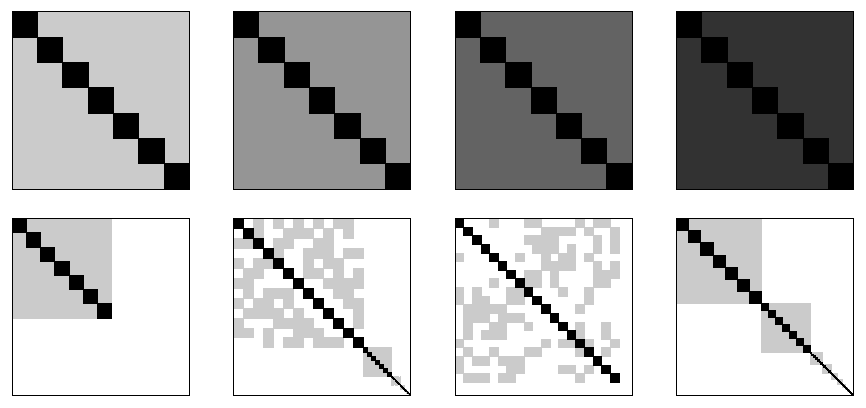
\includegraphics{Graphics/graphons.pdf}
	\end{center}
	\caption{Optimal graphons for induced-$K_{1,8}$-free graphs of fixed edge density. The top row shows the unique optimal graphons of edge densities $\gamma_8\approx0.317$, $\frac{1}{2}$, $\frac{2}{3}$, and $\frac{5}{6}$. The bottom row shows examples of optimal graphons of edge density $\frac{1}{10}$. The white areas represent density 0, gray areas density $p_\gamma\in(0,1)$, and black areas density 1.}
	\label{fig:graphons}
\end{figure}

The next theorem shows that the induced-$H$-free fixed-density variational problem does \emph{not} necessarily exhibit a phase transition for general $H$. A graph $G$ is a \emph{split graph} if there is a partition $V(G)=A\cup B$ such that $G[A]$ is an independent set and $G[B]$ is a clique.

\begin{theorem}\label{thm:c4-main}
Fix a constant $\gamma\in(0,1)$ and let $m\sim\gamma\binom{n}{2}$. Almost all induced-$C_4$-free graphs on $n$ vertices and $m$ edges are split graphs. In particular,
\begin{equation}\label{eqn:c4-entropy-main}
\lim_{n\to\infty}\frac{1}{\binom{n}{2}}\log N^\ast_{n,m}(C_4)=\max_{\lambda\in[0,1]}\left\{2\lambda(1-\lambda)\,H\!\left(\frac{\gamma-\lambda^2}{2\lambda(1-\lambda)}\right)\right\}\,,
\end{equation}
where the maximum is over $\lambda$ for which the right-hand side is well-defined.
\end{theorem}

The right-hand side of \eqref{eqn:c4-entropy-main} is an analytic function of $\gamma\in(0,1)$, reflecting the absence of a phase transition. \Cref{thm:c4-main} resolves the dense case of a conjecture of \citeauthor{morris2024asymmetric} \cite[Conjecture~6.1]{morris2024asymmetric} and refines the theorem of \citeauthor{promel1991excluding} \cite{promel1991excluding} stating that almost all induced-$C_4$-free graphs are split graphs.

\subsection{Overview of proofs}\label{subsec:overview}
Our starting point is the graphon variational problem \eqref{eqn:var-prob-intro-gamma}. We solve \eqref{eqn:var-prob-intro-gamma} via a reduction to an extremal problem over 3-edge-colored graphs. This extremal problem is closely related to prior literature discussed in \Cref{subsec:edit-distance}. We summarize the reduction here.

First, \Cref{lemma:UFHatGraphonSeq} shows that a graphon that is feasible for \eqref{eqn:var-prob-intro-gamma} is the limit of a sequence of \emph{types} $T$ of induced-$K_{1,k}$-free graphs. A type is an $\epsilon$-regular partition equipped with a 2-vertex-colored, 3-edge-colored graph $J$ that encodes whether clusters and pairs of clusters have density close to 0 (green), 1 (blue), or an intermediate value (red). If $T$ is a type for an induced-$K_{1,k}$-free graph, then the induced embedding lemma implies there is no induced homomorphism from $K_{1,k}$ into $J$, written $K_{1,k}\nHookrightarrow J$. If $0\leq d_{ij}\leq1$ represents the density between clusters $i$ and $j$ for all $1\leq i<j\leq\ell$, then the number of induced-$K_{1,k}$-free graphs of edge density $\gamma+o(1)$ that are consistent with $T$ and $\{d_{ij}\}_{1\leq i<j\leq\ell}$ is $e^{o(n^2)}\prod_{i<j}\binom{(n/\ell)^2}{d_{ij}(n/\ell)^2}$. For a fixed type $T$, if the logarithm of this quantity is near-maximum then concavity of the entropy implies the densities $d_{ij}$ corresponding with red pairs $ij$ are nearly equal to one another. The common value of these $d_{ij}$ is $(\gamma\binom{\ell}{2}-e_\blue(J))/e_\red(J)+o(1)$, where $e_\red(J)$ and $e_\blue(J)$ are the numbers of red and blue edges of $J$, respectively.

This motivates the following finite objective. For a 3-edge-colored graph $J$ on $\ell$ vertices with $e_\red(J)>0$, define
\begin{equation}\label{eqn:overview-fgamma}
f_\gamma(J):=e_\red(J)\cdot H\!\left(\frac{\gamma\binom{\ell}{2}-e_\blue(J)}{e_\red(J)}\right)\,.
\end{equation}
Up to the normalizing factor $2/\ell^2$ and a $o(1)$ error, the entropy contribution of a type with colored graph $J$ is governed by $f_\gamma(J)$. Consequently, solving the graphon variational problem reduces to proving extremal and stability results for $f_\gamma(J)$ over colored graphs $J$ satisfying $K_{1,k}\nHookrightarrow J$.

For excluded induced stars, we first prove stability for the linear extremal inequality
\begin{equation}\label{eqn:overview-ineq}
e_\red(J)\leq (k-2)e_\blue(J)+O_k(\ell)\,.
\end{equation}
That is, we prove that every $J$ with $K_{1,k}\nHookrightarrow J$ satisfies \eqref{eqn:overview-ineq} and, moreover, every $J$ for which \eqref{eqn:overview-ineq} is met with near equality is close in Hamming distance to an explicit extremal structure. Passing back to graphons, this gives the constraint $|R_W|\leq (k-2)|O_W|$, where $R_W=\{0<W<1\}$ and $O_W=\{W=1\}$. Jensen's inequality then reduces \eqref{eqn:var-prob-intro-gamma} to a two-variable calculus problem in $|R_W|$ and $|O_W|$, whose solution is $\sE_k(\gamma)$, and whose optimizers satisfy $|R_W|=(k-2)|O_W|$. The proofs of \eqref{eqn:overview-ineq} and the stability of the extremal structure use symmetrization, a local \erdos{}--Simonovits stability step, and an iterative extraction of reduced $(k-2)$-regular components. The extremal structure for \eqref{eqn:overview-ineq} is reflected in the graphons in \Cref{fig:graphons}. For induced-$C_4$-free graphs, we directly prove stability of the objective $f_\gamma(J)$ for every fixed $\gamma\in(0,1)$; in this case, the stable extremal structures are split colorings.

The entropy density and rough structure of fixed-density induced-$H$-free graphs follow from the solution to the graphon variational problem. The finer typical structure assertions require estimates beyond the leading entropy. For excluded induced stars, we first choose a vertex partition minimizing the number of edits needed to obtain the prescribed structure, following the counting approach of \cite{balogh2020efficient,perkins2025typical}. Missing edges inside clique parts and edges between parts that should be nonadjacent are called \emph{defects}. We bound the number of graphs with defects and then compare the counts for the remaining candidate structures.

In \Cref{sec:supercritical}, the partition consists of $k-1$ main parts and a remainder. Optimality excludes high defect degrees. A vertex of intermediate defect degree gives many potential induced stars, whose exclusion incurs a factor $e^{-cn^2}$. When all defect degrees are small, a matching of $h$ defects gives a factor $e^{-chn}$. Janson's inequality supplies these bounds, which outweigh the choices of defects. Holding the remainder graph fixed, we therefore compare with graphs in which the main parts are cliques and have no edges to the remainder. Above $\gamma_k$, absorbing a remainder of size $s$ into a main part increases the count by a factor at least $e^{csn}$. This outweighs the choices of the remainder vertices and proves that almost every graph is co-$(k-1)$-partite.

At the critical density, the linear term in the completion-count comparison vanishes, and the second-order term becomes decisive. In \Cref{sec:critical}, we use the same defect estimates and count the remaining graphs according to their remainder size $s$. For $\gamma=\gamma_k+a\log n/n$ and $s=O(\log n)$, the base-2 logarithm of this count relative to the co-$(k-1)$-partite count is
$$\left(1-\frac{a}{a_\ast}\right)s\log n-\frac{\gamma_k}{a_\ast}s^2+o((\log n)^2)\,,$$
where $a_\ast$ is as in \Cref{thm:main-almostall} \ref{item:thm:main-critical}. Choosing the remainder vertices supplies the $s\log n$ term, while a second-order expansion of the binomial completion count supplies the other two terms. The rate function controls the weighted count of graphs inside the remainder. A quadratic tail bound excludes larger remainders, and maximizing the displayed expression gives the asserted first-order asymptotics. Above $a_\ast$, a further comparison for small positive $s$ shows that the remainder is empty with high probability.

In \Cref{sec:subcritical}, the optimal graphon may have many components. We retain a finite collection of components carrying all but a small amount of the edge density and include the others in the remainder. A \emph{profile} records the local neighborhood data of vertices with many defects and the matching number of the remaining defect graph. If a vertex is adjacent to an intermediate fraction of one part, it must be adjacent to almost all of a neighboring part in the reduced graph. Induced-star-freeness also bounds the number of parts in which the vertex has substantial degree. These restrictions let the losses from almost-complete neighborhoods compensate for the choices of intermediate-density neighborhoods. Combining the edge-count comparison with binomial tail estimates gives a uniform loss per exceptional vertex; in the only configuration where this bound could be tight, optimality of the partition forces a strictly positive relative-entropy loss. The remaining defects have small degrees and are handled by the matching argument and Janson's inequality.

To select the typical subcritical optimizer, we compare these counts with those near the one-component graphon $W^\ast$ on the lower-left of \Cref{fig:graphons}. This graphon leaves the most vertices available for the sparse remainder. Any optimizer a fixed positive cut distance away leaves $\Theta(n)$ fewer such vertices in the comparison. On the additional vertices, inserting a matching gives $e^{\Theta(n\log n)}$ choices. The entropy bound makes each candidate core count at most $e^{O(n)}$ times the reference core count. Transferring $O(n)$ edges from the core to the remainder to preserve the total edge count also costs only $e^{O(n)}$, as do the choices of vertex partitions. This proves concentration at $W^\ast$. We then use the defect estimates and control the multiplicity of clique covers to obtain the exact decomposition in \Cref{thm:main-almostall} \ref{item:thm:main-almostall-sub}. A further matching comparison on isolated remainder vertices gives the linear lower bound on its number of edges.

\subsection{Related work}
\subsubsection{Coloring number and criticality.}\label{subsec:col-num}
The \emph{coloring number} $\tau(H)$ is the least integer $q$ such that, for every pair of nonnegative integers $s,t$ with $s+t=q$, the vertices of $H$ can be partitioned into $s$ cliques and $t$ independent sets. For $\tau(H)\geq3$, \citeauthor{balogh2011excluding} \cite{balogh2011excluding} proved a criticality criterion for almost every induced-$H$-free graph to admit a partition into $s$ cliques and $t$ independent sets, where $s+t=\tau(H)-1$ and $H$ admits no such partition. This is the induced analogue of the characterization by \citeauthor{promel1992asymptotic} \cite{promel1992asymptotic} of non-bipartite graphs $H$ for which almost all $H$-free graphs are $(\chi(H)-1)$-partite. These results concern graphs without a prescribed edge count. In the fixed-density setting studied here, even for excluded induced stars, the typical structure depends on the density and can include a nonempty sparse remainder.

\subsubsection{Edit distance and hereditary properties.}\label{subsec:edit-distance}
Our work is related to literature on extremal problems for multigraphs, most notably by \citeauthor{marchant2010extremal} \cite{marchant2010extremal,marchant2011structure} and \citeauthor{thomason2011graphs} \cite{thomason2011graphs}. This literature focuses on calculating an extremal parameter $\kappa_p$ that is analogous to the Tur\'an density. Theorem 4.4 in \cite{marchant2010extremal} shows how to convert between $\kappa_p$ and the large deviation rate function for a hereditary property in $G(n,p)$. Consequently, these results determine the large deviation rate function for induced-$H$-freeness for several specific graphs $H$. For excluded induced stars, \citeauthor{thomason2011graphs} \cite[Section~7.5]{thomason2011graphs} exhibits infinitely many colored extremal structures at $p=p_k$, consistent with the graphon optimizer family in \Cref{thm:gnp-graphons}. Our work differs from this previous literature in that we focus mainly on the fixed-density setting, characterize all graphon optimizers for both models, and prove finer typical structure results.

\subsubsection{Other density-constrained models}
Numerous prior works have studied typical structure and phase transitions in random graph models defined by subgraph density constraints. A well-studied case is the uniformly random graph of given edge and triangle density; several works have characterized optimal graphons in subsets of the feasible region of densities and proven the existence of phase transitions \cite{radin2013phase,radin2014asymptotics,radin2015singularities}. The main variational problem studied here imposes zero induced-star density. Allowing a small positive induced-star density leads to the question in \Cref{conj:relaxed-star-exclusion}: whether this relaxation selects the same one-component graphon as the lower-order counting argument, despite the existence of infinitely many optimizers under exact exclusion.

\subsection{Future directions}
A natural extension is to allow a small positive density of induced stars. For $k\geq3$, $\gamma\in(0,1)$, and $\epsilon\geq0$, define
$$\Phi_k(\gamma,\epsilon):=\sup\left\{H(W):W\in\cW\,,\,t(K_2,W)=\gamma\,,\,t_\ind(K_{1,k},W)\leq\epsilon\right\}\,,$$
where $H(W):=\int_{[0,1]^2}H(W(x,y))\,dx\,dy$. Our results give $\Phi_k(\gamma,0)=\sE_k(\gamma)$ and infinitely many optimizers when $\gamma<\gamma_k$. We conjecture that allowing a vanishing induced-star density selects the same one-component graphon as the finite counting argument.

For $\gamma\in(0,\gamma_k)$, put $\mu:=\sqrt{\gamma/\gamma_k}$ and $s:=1-\mu$. Let $W^\ast$ be the graphon obtained by rescaling $W^\ast_{\gamma_k}$ from \eqref{eqn:opt-graphon-super} to $[0,\mu]^2$ and setting it equal to zero elsewhere.

\begin{conjecture}\label{conj:relaxed-star-exclusion}
Fix $k\geq3$ and $\gamma\in(0,\gamma_k)$. As $\epsilon\downarrow0$,
$$\Phi_k(\gamma,\epsilon)=\sE_k(\gamma)+\left(\frac{s^{(k-1)/k}}{k}+o(1)\right)\epsilon^{1/k}\log\frac1\epsilon\,.$$
Moreover, every choice of optimizing graphons $W_\epsilon$ satisfies
$$\delta_\square(W_\epsilon,W^\ast)\longrightarrow0\,.$$
\end{conjecture}

The proposed entropy correction is attained to leading order by putting a small constant density $q$ on the isolated remainder of $W^\ast$ and shrinking its nonzero component to preserve edge density $\gamma$. The induced-star density is then asymptotic to $s^{k+1}q^k$, while the entropy gain is $s^2q\log(1/q)+O_{k,\gamma}(q)$. The conjecture concerns the leading correction and limiting graphon, rather than the exact form of an optimizer for positive $\epsilon$; smaller perturbations inside the clique parts may further increase the entropy.

\subsection{Organization}
In \Cref{sec:prelim}, we include background on colored graphs, regularity, graphons, and cut metric that will be used throughout the paper. In \Cref{sec:graphon-prob}, we solve the graphon variational problems, fully characterizing all optimizers. In \Cref{sec:entropy} we prove \Cref{thm:main-entropy,thm:main-rate,thm:ent-graphons,thm:gnp-graphons}. In \Cref{sec:supercritical,sec:critical,sec:subcritical}, we prove \Cref{thm:main-almostall} \ref{item:thm:main-almostall-super}, \ref{item:thm:main-critical}, and \ref{item:thm:main-almostall-sub}, respectively. In \Cref{sec:erdosrenyi}, we prove \Cref{thm:gnp-typ-struc}. In \Cref{sec:edge-coloring}, we establish the extremal and stability results for edge colorings that underlie the graphon analysis. In \Cref{sec:deferred}, we give deferred proofs from the earlier sections. Finally, in \Cref{sec:c4-free} we prove \Cref{thm:c4-main}.
